\subsection{Offloading Nodes via Network Wrapper}\label{subsec:networkoffloading}

For computationally intensive tasks (e.g., ML-based nodes), mobile devices may lack sufficient compute capacity.
MotionDAG supports partial offloading of motion processing stages to a remote server without altering the core DAG API. 
This is enabled by the \textit{Network Wrapper}, a mechanism that encapsulates selected motion nodes for remote execution while preserving pipeline semantics and node composition. Computationally intensive nodes--such as inverse kinematics solvers or learning-based estimators--can be selectively wrapped and delegated to a centralized server, which acts as a processing hub and transmits results back to the client. Offloading is optional and transparent to the rest of the graph; only resource-constrained nodes need to be wrapped.

The wrapper intercepts input subscriptions of the node and redirects relevant pose streams to the server for remote computation. 
Crucially, it determines the appropriate synchronization strategy based on the runtime placement of the node's publishers and subscribers. The wrapper applies one of four synchronization policies:

\begin{itemize}
    \item \textbf{Client-to-Client:}
    Both publisher and subscriber reside on the same device. No network action is required; local data flow proceeds as usual.
    \item \textbf{Client-to-Server:} 
    Inputs are replicated to the server; computation runs server-side. The server buffer becomes the source for downstream server nodes; results are optionally replicated back to the client.
    \item \textbf{Server-to-Server:} 
    Both the publisher and subscriber are wrapped and reside on the server. All data exchange and computation occur on the server, eliminating the need for network synchronization with any client.
    \item \textbf{Server-to-Client:} 
    The publisher is network-wrapped and on the server, and the subscriber is on a client. The server pushes outputs to the client via unicast RPC at the subscriber's cadence.
\end{itemize}

Interaction latency and throughput across representative client-server configurations are evaluated in \hyperref[subsec:network-offloading-eval]{Network Offloading Performance}, demonstrating that our offloading mechanism sustains real-time performance under practical network conditions.


\begin{figure*}[t]
  \centering
  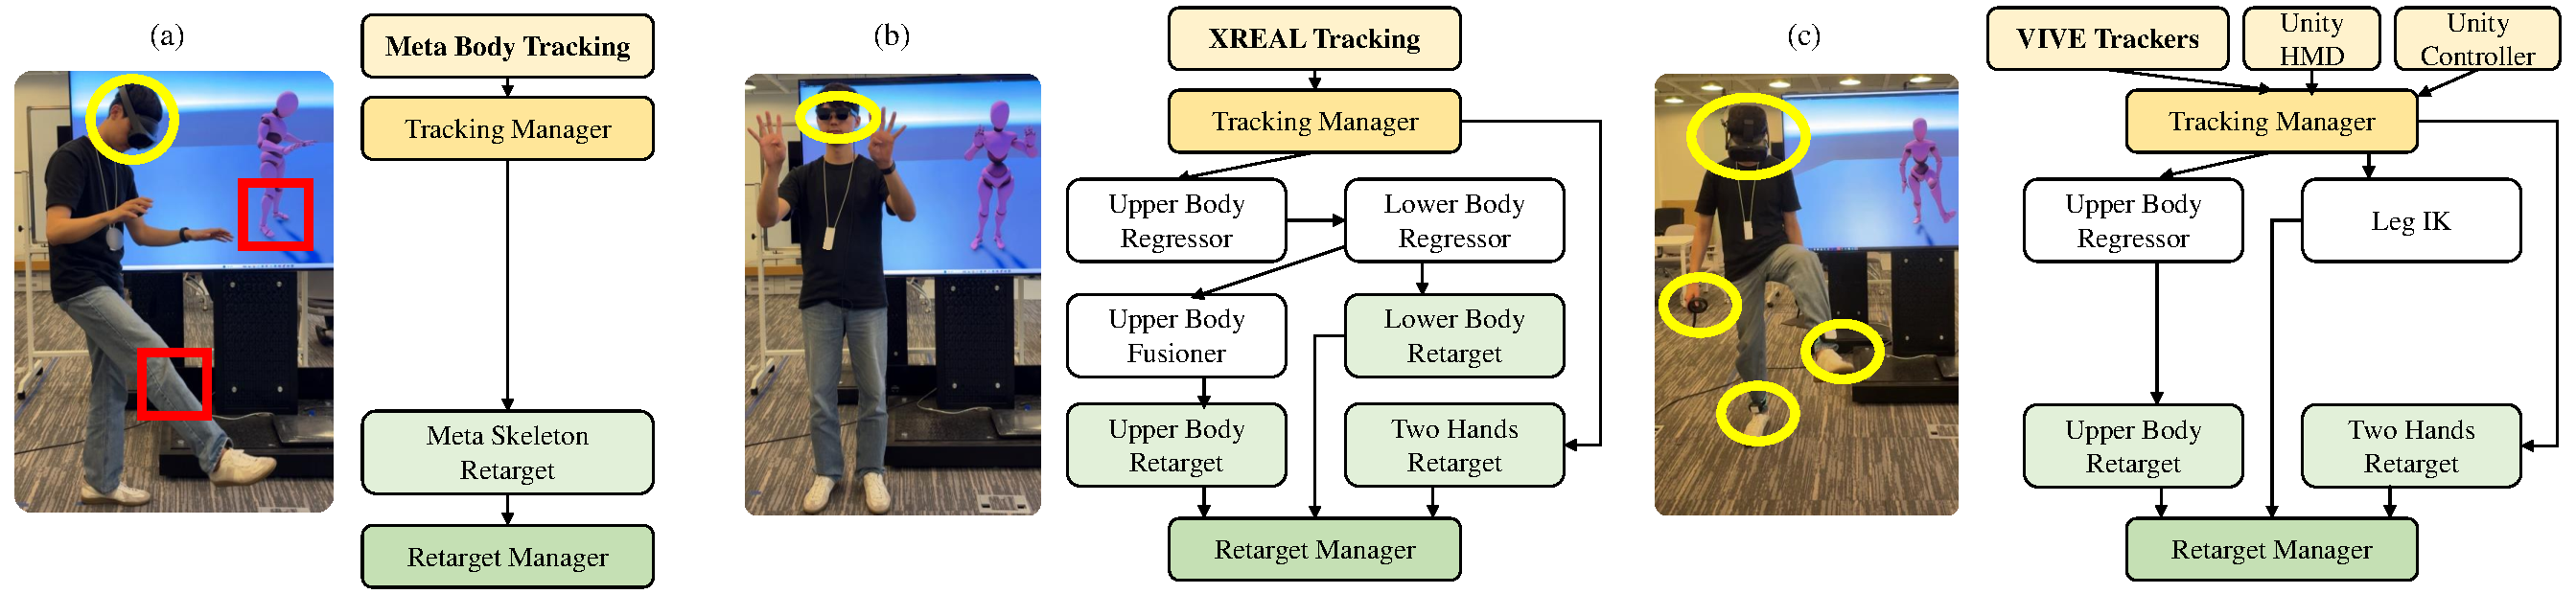
\includegraphics[width=\linewidth]{figures/fig5-configure.pdf}
  \caption{Our framework standardizes diverse tracking inputs into unified pose streams, processes motion via composable nodes, and retargets to a custom avatar.
We present three representative full-body pipelines: (a) Meta body tracking, (b) XREAL AR glasses with hand tracking, and (c) Vive HMD with controllers and physical trackers.}
  \label{fig:teaser}
\end{figure*}
